\documentclass[tikz=true]{standalone}
\usepackage{graphicx, standalone}
\usepackage[compat=1.1.0]{tikz-feynman}
\usepackage{tikz}
\usepackage{amsmath, amssymb}
\usepackage{euler}
\usepackage{fontspec}
\setmainfont{MinionPro}

\renewcommand{\k}{\ensuremath\text{k}}
\newcommand{\kp}{\ensuremath\text{k}'}
\newcommand{\q}{\ensuremath\text{q}}

\begin{document}

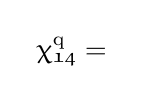
\begin{tikzpicture}[baseline=(current bounding box.center)]
    \node {$\chi_{\mathfrak{14}}^{\q}=$};
\end{tikzpicture}
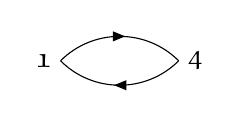
\begin{tikzpicture}[baseline=(current bounding box.center)]
	\begin{feynman}
		\vertex (a1);
		\vertex[right=of a1] (a2);
		
		\node[left=0em of a1] {$\mathfrak{1}$};
		\node[right=0em of a2] {$\mathfrak{4}$};
		
		\diagram* {
			(a1) -- [fermion, bend left=45, arrow size=1pt] (a2) -- [fermion, bend left=45, arrow size=1pt] (a1)
		};
	\end{feynman} 
\end{tikzpicture}
\begin{tikzpicture}[baseline=(current bounding box.center)]
    \node {$-$};
\end{tikzpicture}
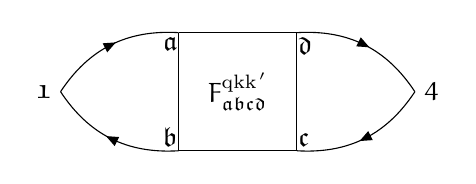
\begin{tikzpicture}[baseline=(current bounding box.center)]
	\begin{feynman}
		\vertex (b1);
		\vertex[below=of b1] (b2);
		\vertex[right=of b1] (c1);
		\vertex[right=of b2] (c2);
		
		\path (b1) -- (b2) coordinate[midway] (i);
		\vertex[left=of i] (a);
		
		\path (c1) -- (c2) coordinate[midway] (j);
		\vertex[right=of j] (d);
		
		\node (content) at ($(b1)!0.5!(c2)$) {$F_{\mathfrak{abcd}}^{\q\k\kp}$};
		
		\node[left=0em of a] {$\mathfrak{1}$};
		\node[right=0em of d] {$\mathfrak{4}$};
		
		\def\sc{1.0};
		
		\node[below left=-0.2em and -0.3em of b1] {\scalebox{\sc}{$\mathfrak{a}$}};
		\node[above left=-0.2em and -0.3em of b2] {\scalebox{\sc}{$\mathfrak{b}$}};
		\node[below right=-0.2em and -0.3em of c1] {\scalebox{\sc}{$\mathfrak{d}$}};
		\node[above right=-0.2em and -0.3em of c2] {\scalebox{\sc}{$\mathfrak{c}$}};
		
		\diagram* {
			(a) -- [fermion, bend left=30, arrow size=1pt] (b1),
			(b2) -- [fermion, bend left=30, arrow size=1pt] (a),
			(c1) -- [fermion, bend left=30, arrow size=1pt] (d),
			(d) -- [fermion, bend left=30, arrow size=1pt] (c2),
			(b1) -- (b2) -- (c2) -- (c1) -- (b1),		
		};	
	\end{feynman} 
\end{tikzpicture}

\end{document}